\documentclass[a4paper,12pt]{article}

\usepackage[slovene]{babel}
\usepackage{amsfonts,amssymb,amsmath}
\usepackage[utf8]{inputenc}
\usepackage[T1]{fontenc}
\usepackage{lmodern}
\usepackage{graphicx}
\graphicspath{{./imgs/}}
\usepackage{url}

\def\N{\mathbb{N}} % mnozica naravnih stevil
\def\Z{\mathbb{Z}} % mnozica celih stevil
\def\Q{\mathbb{Q}} % mnozica racionalnih stevil
\def\R{\mathbb{R}} % mnozica realnih stevil
\def\C{\mathbb{C}} % mnozica kompleksnih stevil
\def\H{\mathbb{H}} % mnozica kvaternionov
\def\E{\mathbb{E}} % evklidski prostor 
\def\Qe{\textbf{Q}_{e}} % mnozica versorjev
\def\Ue{\textbf{U}_{e}} % mnozica pravih versorjev
\def\1{\textbf{\emph{1}}}
\newcommand{\geslo}[2]{\noindent\textbf{#1} \quad \hangindent=1cm #2\\[-1pc]}
\newcommand{\dotpr}[2]{\langle #1, #2 \rangle}
\newcommand{\conj}[1]{\overline{#1}}

\def\qed{$\hfill\Box$}   % konec dokaza
\def\qedm{\qquad\Box}   % konec dokaza v matematičnem načinu
\newtheorem{izrek}{Izrek}
\newtheorem{trditev}{Trditev}
\newtheorem{posledica}{Posledica}
\newtheorem{lema}{Lema}
\newtheorem{opomba}{Opomba}
\newtheorem{definicija}{Definicija}
\newtheorem{zgled}{Zgled}

\title{Rotacije opisane s kvaternioni \\ 
\Large Seminar}
\author{Timotej Mlakar \\
Fakulteta za matematiko in fiziko \\
Oddelek za matematiko}
\date{\today}

\begin{document}


%%%%%%%%%%%%%%%%%%%%%%%%%%%%%%%%%%%%%%%%%%%%%%%%%%%%%%%%%%%%%%%%%%%%%


\maketitle
\vspace{5em}
\tableofcontents


%%%%%%%%%%%%%%%%%%%%%%%%%%%%%%%%%%%%%%%%%%%%%%%%%%%%%%%%%%%%%%%%%%%%%
\newpage
\section{Uvod}

Rotacije prostora $\R^3$ navadno opišemo z linearnimi preslikavami prostora oziroma njim pripadajočimi matrikami.
V splošni uporabi je za opis orientacije objekta tako imenovan \emph{sistem Eulerjevih kotov}. Znameniti \emph{Eulerjev izrek o rotacijah} namreč pravi,
da se da vsako rotacijo opisati s tremi parametri oziroma koti.

Težava nastopi, ko moramo tako rotacijo zapisati. Za vsakega od kotov potrebujemo svojo preslikavo, ki jo
nato komponiramo z drugima dvema, da dobimo končno preslikavo:
\begin{center}
   $R = R_{1}R_{2}R_{3}$,
\end{center}
kjer je $R$ končna rotacija, $B, C, D$ pa so rotacije posameznih ravnin glede na želeni kot/parameter.
Za elemente matrike, ki pripada R, potrebujemo 9  podatkov \cite{salamin1979application}, ki jih izračunamo z matričnim množenjem.

Težava je, da je tako računanje časovno zelo zahtevno, zato bomo izpeljali drug, bolj učinkovit našin opisovanja takih transformacij.

Za motivacijo uporabimo analog rotacij v dveh dimenzijah, in sicer množenje kompleksnih števil.
Spomnio se, da množenje kompleksnega števila $z$ z enotskim komplekstim številom $e^{i\theta}$ zavrti $z$ okoli koordinatnega izhodišča za kot $\theta$.
Podobno bi želeli narediti v 3-razsežnem prostoru, vendar za to potrebujemo množenje.
Ta problem je rešil Sir William Rowan Hamilton \cite{shoemake1985animating}, ko je oktobra leta 1843 na mostu Brougham Bridge dognal identitete za množenje v 4-razsežnem prostoru.
Ta ugotovitev je bila tako odmevna, da je trenutek za vedno zabeležen v kamnu na mostu, kjer je vklesano
\begin{center}
   \emph{ Here as he walked by
   on the 16th of October 1843
   Sir William Rowan Hamilton
   in a flash of genius discovered
   the fundamental formula for
   quaternion multiplication}\\
   $i^2 = j^2 = k^2 = ijk = -1$\\
   \emph{ \& cut it on a stone of this bridge}. ~\cite{baez2004baezstuff}
\end{center}

Ekvivalentno Eulerjevim kotom s pomočjo kvaternionov dobimo tako imenovane \emph{Eulerjeve parametre}, s katerimi
lahko poljubno rotacijo/orientacijo opišemo samo s štirimi parametri. Prav tako je za večkratno apliciranje preslikav rotacij sedaj
potrebnih veliko manj operacij. To nas motivira, da predpise preslikav rotacij zapišemo s kvaternionskim množenjem.
\newpage

%%%%%%%%%%%%%%%%%%%%%%%%%%%%%%%%%%%%%%%%%%%%%%%%%%%%%%%%%%%%%%%%%%%

\section{Kvaternionska algebra}
\subsection{Definicije in oznake}

\begin{definicija}
Naj bo $V$ $4$-razsežen vektorski prostor nad $R$. Izberemo bazo $\left\{\1, i, j, k\right\}$. Elementi $V$ so oblike $\textbf{q} = q_{0}\1 + q_{1}i + q_{2}j + q_{3}k = q_{0} + \vec{q}$, imenujemo jih \emph{kvaternioni}.
Vektorski prostor $V$ opremimo z operacijo množenja tako, da definiramo množenje njegovih baznih elementov, in sicer
\begin{center}
   $\1 \1 = \1, \hspace{1em}  \1i = i, \hspace{1em} \1j = j, \hspace{1em} \1k = k,$\\
   $ij = k, \hspace{1em} jk = i, \hspace{1em} ki = j,$\\
   $i^2 = j^2 = k^2 = ijk = -1\1$.
\end{center}

Naj bosta $p, q \in \H$. Definiramo seštevanje in množenje s skalarjem kot običajno
\begin{center}
   $p + q = \left( p_{0} + q_{0} \right) + \left( \vec{p} + \vec{q} \right)$, \\
   $ \lambda q = \lambda \left(q_{0} + \vec{q} \right) = \lambda q_{0} + \left(\lambda \vec{q}\right) $.
\end{center}
Prav tako definiramo običajno množenje v skladu z definicijo množenja baznih elementov. Tedaj lahko
produkt $pq$ napišemo kot
\begin{center}
   $pq = (p_{0} q_{0} - \vec{p} \vec{q}) + (p_{0}\vec{q} + q_{0}\vec{p} + \vec{p}\times\vec{q})$,
\end{center}
kjer je $\vec{p}\vec{q}$ običajni skalarni produkt v $\R^3$.
Tedaj $V$ postane $4$-razsežna algebra nad $\R$, označimo $\H$ in jo imenujemo \emph{Kvaternionska algebra}.\emph{~\cite{dam1998quaternions}}
\end{definicija}
\begin{opomba}
Za $p,q \in \H, \lambda \in \R$ velja
\begin{center}
      $(\lambda p)q = p(\lambda q) = \lambda (pq)$.
\end{center}
\end{opomba}
\begin{definicija}
Naj bo $q = q_{0} + \vec{q}\in \H$. S $\overline{q} = q_{0} -\vec{q}$ označimo \emph{konjugirani kvaternion} q.
\end{definicija}
Velja, da je $q\overline{q} \in \R$. Tako lahko definiramo še 
\begin{center}
   $q^{-1} = \dfrac{1}{q\overline{q}} \overline{q}$.
\end{center}
Prav tako lahko vidimo da je $\overline{p \cdot q} = \overline{q} \cdot \overline{p}$. Ker množenje kvaternionov ni komutativno,
v splošnem $\overline{pq} \neq \overline{qp}$. Ker je $\H$ algebra, je na njej smiselno definirati skalarni produkt.

\break
\begin{definicija}
Naj bosta $p,q \in \H$. Definiramo skalarni produkt kvaternionov
\begin{center}
   $\dotpr{p}{q} = \frac{1}{2} (\overline{p}q + \overline{q}p)$.\emph{~\cite{weiner2005quaternions}}
\end{center}
Norma porojena s skalarnim produktom je tedaj
\begin{center}
   $|q| = ||q|| = \sqrt{\dotpr{q}{q}}$.
\end{center}
\end{definicija}

\begin{opomba}
Iz definicije skalarnega produkta takoj sledi $\langle q, q\rangle = q\overline{q} = \overline{q}q$.
Podobno kot absolutna vrednost na $\R$ in $\C$ je norma na kvaternionih multiplikativna.
\end{opomba}
Za poljubna $p,q \in \H$ torej velja $|pq| = |p||q|$. Oglejmo si $|pq|^2$
\begin{center}
   $|pq|^2 = \langle pq, pq \rangle = pq\overline{pq}$.
\end{center}
Spomnimo se, da $\overline{p \cdot q} = \overline{q} \cdot \overline{p}$. Torej je
\begin{center}
   $pq\overline{pq} = p\cdot q\cdot \overline{q} \cdot \overline{p} = p |q|^2 \overline{p}$.
\end{center}
Ker je $|q|^2$ skalar, pri množenju komutira s kvaternioni. Torej
\begin{center}
   $p|q|^2\overline{p} = |q|^2p\overline{p} = |q|^2 |p|^2 = |p|^2 |q|^2$.
\end{center}
Sledi torej $|pq| = |p||q|$. ~\cite{weiner2005quaternions}

Podobno kot pri rotaciji kompleksne ravnine, kjer množimo s števili iz enotske krožnice, tukaj potrebujemo 
enotske kvaternione.

\begin{definicija}
   Naj bo $q \in \H$. Kvaternion q imenujemo \emph{versor} oziroma \emph{enotski kvaternion}, če velja
   $|q| = 1$. Množico versorjev označimo s $\Qe$

   Če za $u \in \H $ velja $u = \vec{u}$ in $|u| = 1$, kvaternion u imenujemo \emph{čisti} oziroma \emph{pravi} versor.
   Množico pravih versorjev označimo z $\Ue$.

   Z $\R$ od tu naprej označujemo $\{ q \in \H; \vec{q} = 0 \}$ množico skalarnih kvaternionov, podobno od tu naprej z $\R^3$ označujemo
   množico čistih kvaternionov $\{q \in \H; q_{0} = 0 \}$. \emph{~\cite{weiner2005quaternions}}
\end{definicija}
%%%% TUKI SE NEKI MANKA SAM NEVEM KAJ TOCN
\begin{opomba}
   Za čista versorja $u, v \in \Ue$ velja, da 
   \begin{center}
      $\dotpr{u}{v} = 0 \iff uv + vu = 0$.
   \end{center}
\end{opomba}
Naj bosta $u, v \in \Ue$. Za poljuben versor iz $\Ue$ velja $\overline{u} = -u$. Pogledamo $\dotpr{u}{v}$ :
\begin{center}
   $\dotpr{u}{v} = \frac{1}{2}(\overline{u}v + \overline{v}u) = \frac{1}{2}(-uv -vu) = -\frac{1}{2}(uv + vu)$.
\end{center}
Od tu sledi da $\dotpr{u}{v} = 0 \iff uv + vu = 0$.

Tukaj opomnimo še naslednje: naj bo $u \in \Ue$. Ker $|u| = 1$ sledi, da je $u$ neničeln kvaternion.
Ker je $\Ue \subset \H$ in je $\H$ algebra, je vsak neničenli kvaternion obrnljiv. Vemo torej, da obstaja tak $u^{-1}$ da je
\begin{center}
   $uu^{-1} = 1$.
\end{center}
Ker je za poljuben $q \in \H, q^{-1} = \dfrac{1}{\overline{q}q} \overline{q}$, za $u \in \Ue$ pa velja $u\overline{u} = |u|^2$, je 
\begin{center}
   $u^{-1} = \dfrac{\overline{u}}{|u|^2} = \dfrac{-u}{1} = -u$.
\end{center}
Če združimo ti dve dejstvi, velja še naslednja enakost:
\begin{center}
   $uu^{-1} = -uu = -u^2 = 1 \Rightarrow u^2 = -1$.
\end{center}

\subsection{Zapis  kvaternionov v polarni obliki}

Podobno kot kompleksna števila lahko kvaternione zapišemo v polarni obliki. T.j.
kompleksno število $z = \text{x} + i\text{y}$ lahko zapišemo kot $|z|( \cos\theta + i\sin\theta )$. Z \emph{eulerjevo formulo} lahko to kompleksno število
zapišemo kot $z = e^{i\theta}$.

V kompleksni ravnini je ta zapis dobro definiran, saj imamo le eno kompleksno enoto $i$.
V kvaternionih pa imamo celo množico čistih enotskih kvaternionov $\Ue$, s katerimi lahko zapišemo kvaternion.

\begin{trditev}
Naj bo $q \in \Qe$. Tedaj obstajata $\theta \in \R$ in $u \in \Ue$, da je
\begin{center}
   $q = \1\cos\theta + u\sin\theta$.
\end{center}
\end{trditev}


\noindent
{\em Dokaz: \/}Enakost pokažemo za enotske kvaternione, saj poljuben kvaternion lahko dobimo kot produkt enotskega s skalarjem.
Naj bo $q = q_{0} + \vec{q} \in \Qe$. Ker sta $q_{0}$ in $\vec{q}$ glede na definirani skalarni produkt pravokotna, opazujemo trikotnik s katetama dolžine $q_{0}$ in $|\vec{q}|$, ter hipotenuzo dolžine 1.
Definiramo $\theta := \arccos(q_{0})$. Tu dopuščamo, da je $q_{0}$ tudi negativen, ali pa enak $\pm 1$. Tedaj je $\vec{q} = u\sin\theta$ za nek $u \in \Ue$, ki kaže v smeri $\vec{q}$.
Velja torej
\begin{center}
   $q = q_{0} + \vec{q} = \cos\theta + u\sin\theta$.
\end{center}
\qed

\noindent Dokaz je povzet po Lyonsu. \cite{2021Quaternions}
\begin{opomba}
Opazimo, da nam trditev zagotavlja \emph{le obstoj} in ne enoličnosti.
\end{opomba}
\break
Preprost protiprimer za enoličnost je $q \in \Qe, q = \1\cos\theta + u\sin\theta$.
Pogledamo $\theta' = -\theta$ in $u' = \conj{u} = -u$. Tedaj je
\begin{center}
   $\1\cos\theta' + u'\sin\theta' = \1\cos(-\theta) -u\sin(-\theta) = \1\cos\theta + u\sin\theta = q$.
\end{center}
Vidimo, da ima q torej $2$ zapisa. Podobno sklepanje ponovimo za kvaternion 0. Za kvaternion 0 v enakosti zadoščata vsaka $u \in \Ue$ in $\theta \in \R$, saj je 0 možno dobiti le z množenjem enotskega kvaterniona
s skalarjem 0.
   
Zaradi lažjega računanja bomo polarni zapis kvaternionov spremeniti v eksponentni zapis. Spet se najprej spomnimo kompleksne ravnine, kjer lahko
vsak $z \in \C$ zapišemo kot $|z|e^{i\varphi}$ za nek $\varphi \in \R$. To naredimo, saj je tako
algebraična manipulacija kompleksnih izrazov lažja.

Vzamemo Taylorjev razvoj $e^t$:
\begin{center}
   $e^t = 1+t+\dfrac{t^2}{2}+\dfrac{t^3}{6}+\dfrac{t^4}{24} + \cdots$.
\end{center}
V Taylorjev razvoj vstavimo $t = u\theta, u \in \Ue, \theta \in \R$. Dobimo %Tukej obrazlozi zakaj to lahko nardimo
\begin{center}
   $e^{u\theta} = 1 + u\theta + \dfrac{(u\theta)^2}{2} + \dfrac{(u\theta)^3}{6} + \dfrac{(u\theta)^4}{24} + \cdots$.
\end{center}
Spomnimo se, da ker je $u \in \Ue$, velja $u^2=-1$. Ker $e^t$ konvergira enakomerno povsod, lahko vrsto preuredimo, in sicer:
\begin{center}
   $1 + u\theta + \dfrac{(u\theta)^2}{2} + \dfrac{(u\theta)^3}{6} + \dfrac{(u\theta)^4}{24} + \cdots = (1 + \dfrac{(u\theta)^2}{2} + \dfrac{(u\theta)^4}{24}+ \cdots) + (u\theta + \dfrac{(u\theta)^3}{6} + \cdots) = $
   $(1-\dfrac{\theta^2}{2}+\dfrac{\theta^4}{24}- \cdots) + u(\theta - \dfrac{\theta^3}{6} +\dfrac{\theta^5}{120} - \cdots)$
\end{center}
V levem in desnem oklepaju vidimo Taylorjev razvoj funkcij $\cos$ in $\sin$. Sledi torej
\begin{center}
   $e^{u\theta} = \cos\theta  + u\sin\theta$.
\end{center}
Zgornjo trditev lahko sedaj spremenimo v lepšo obliko, t.j. za vsak $q \in \Qe$ obstajata
$\theta \in \R$ in $u \in \Ue$, da velja $q =  e^{u\theta}$.

\begin{opomba} 
Naj bosta $p,q \in \Qe$. Vemo, da produkt kvaternionov ni komutativen, t. j. $p q \neq q p$. Če p in q zapišemo v polarni obliki, 
$p = e^{u\theta}, q = e^{v\varphi}$, lahko produkta napišemo kot
\begin{center}
   $p q = e^{u\theta} e^{v\varphi}$ in $q p = e^{v\varphi}e^{u\theta}$.
\end{center}
\end{opomba}
Zaradi nekomutativnosti prav tako sledi, da $e^{u\theta} e^{v\varphi} \neq e^{v\varphi}e^{u\theta}$. Če bi tak produkt obstajal, bi v eksponentu imeli primer nekomutativne vsote,
kar pa je seveda v protislovju z definicijo vsote iz algebre $\H$.


Zanima nas, kdaj taki kvaternioni komutirajo.
\begin{trditev}
Naj bosta $p,q \in \Qe$ taka, da $\exists u \in \Ue$, da $p = e^{u\theta}$ in $q = e^{u\varphi}$ za neka $\theta, \varphi \in \R$.
Tedaj je $pq = qp$.
\end{trditev}
\noindent
{\em Dokaz:\/} Zapišemo $p = \cos\theta + u\sin\theta$, $q = \cos\varphi + u\sin\varphi$.
Spomnimo se, da skalarji komutirajo z vsemi kvaternioni. Torej je
\begin{align*}
   pq & = (\cos\theta + u\sin\theta)(\cos\varphi + u\sin\varphi)\\
   & = \cos\theta(\cos\varphi + u\sin\varphi) + u\sin\theta(\cos\varphi + u\sin\varphi)\\
   & = (\cos\varphi + u\sin\varphi)\cos\theta + (u\cos\varphi + u^2\sin\varphi)\sin\theta\\
   & = (\cos\varphi + u\sin\varphi)\cos\theta + (\cos\varphi + u\sin\varphi)u\sin\theta\\
   & = (\cos\varphi + u\sin\varphi)(\cos\theta + u\sin\theta) = qp.
\end{align*}
\qed

Trditev nam pove, da kvaternioni z različnim realnim argumentom in istim versorjem med sabo komutirajo.
Prav tako komutirata kvaterniona, ki sta zapisana s konjugiranima versorjema, saj je to ekvivalentno negativnemu argumentu v polarnem zapisu.

\section{Preslikava rotacije}
\subsection{Preslikava}
\begin{definicija}
Naj bo $q \in \Qe$. Označimo preslikavi $L_{q}, R_{q} : \H \to \H$ levega in desnega množenja:
\begin{center}
   $L_{q}x = qx$, $R_{q}x = xq$.
\end{center}
\end{definicija}

\noindent Vidimo, da sta $L_{q}$ in $R_{q}$ linearni preslikavi. Naj bosta $x,y \in \H$ in $\alpha, \beta \in \R$.
\begin{center}
   $L_{q}(\alpha x +\beta y) = q(\alpha x +\beta y)$.
\end{center}
Uporabimo komutativnost skalarjev in levo distributivnost nad kvaternioni:
\begin{center}
   $q(\alpha x +\beta y) = \alpha qx + \beta qy = \alpha L_{q}x + \beta L_{q}y$.
\end{center}
S podobnim računom pokažemo, da je $R_{q}$ tudi linearna. Poleg tega vidimo, da sta preslikavi ortogonalni,
t.j., da ohranjata skalarni produkt. Iz tega sledi tudi, da sta preslikavi $L_{q}$ in $R_{q}$ izometriji prostora.

\newpage
Ti preslikavi med sabo komutirata, saj za $p,q \in \Qe$ in fiksen $x \in \H$:
\begin{center}
   $(L_{p} \circ R_{q})x = p(xq) = (px)q = (R_{q} \circ L_{p})x$.
\end{center}
Njun kompozitum je prav tako ortogonalna preslikava
Definiramo torej kompozitum preslikav kot posebno preslikavo
\begin{definicija}
Naj bosta $p,q \in \Qe$. S $C: \H \to \H$ označimo kompozitum levega in desnega množenja
\begin{center}
   $C_{p,q} = L_{p} \circ R_{q} = R_{q} \circ L_{p}$.
\end{center}
\end{definicija}
C je za poljubna $p,q \in \Qe$ bijektivna in ortogonarlna. Ortogonalnost sledi iz kompozicije dveh ortogonalnih preslikav,
surjektivnost je očitna. Injektivnost preverimo z uporabo pravil krajšanja v kvaternionski algebri $\H$.
Če je namreč $C_{p,q}x = C_{p,q}y$, je to enako $pxq = pyq$. Ker lahko kvaternione okrajšamo, sledi $x = y$.

Naj bodo $p_1, q_1, p_2, q_2 \in \Qe$. Poglejmo preslikavi $C_{p_1, q_1}, C_{p_2,q_2}$. Če preslikavi komponiramo, je rezultat ponovno preslikava take oblike, t.j.
$C_{p_1 p_2, q_2 q_1}$. Inverz te preslikave je prav tako ortogonalna preslikava, namreč $C^{-1}_{p,q} = C_{p^{-1}, q^{-1}}.$ 
Imamo torej grupo preslikav za komponiranje nad $\Qe$. Izkaže se, da je ta grupa kar grupa avtomorfizmov $\text{Aut} ( \H )$ \cite{brevsar2018skolem}.
Opomnimo samo, da se pri komponiranju teh preslikav vrstni red desnega množenja obrne.

Posebej omenimo množico preslikav oblike $C_{q,\conj{q}}$. Vemo, da se da $q$ zapisati v polarni obliki kot
$\cos\theta + u\sin\theta = e^{u\theta}$ za neka $u \in \Ue, \theta \in \R$. Ker je $q \in \Qe$, je $\conj{q} = e^{-u\theta}$.
Preslikavo $C_{q, \conj{q}}$ je torej možno zapisati kot
\begin{center}
   $Cx := C_{q, \conj{q}} x = e^{u\theta}x e^{-u\theta}$.
\end{center}
Ker je $C$ ortogonalna preslikava, ohranja skalarni produkt. Spomnimo se, da so skalarni kvaternioni in čisti kvaternioni pravokotni,
saj ce $\alpha \in \R$ in $q \in \R^3$, je $\dotpr{\alpha}{q} = \frac{1}{2} (\conj{\alpha}q + \conj{q}\alpha)$. Ker je $\alpha \in \R$, je $\conj{\alpha} = \alpha$.
Torej je dalje skalarni produkt enak $\frac{1}{2}(\alpha q - \alpha q) = 0$. Prostor skalarjev je torej invarianten za preslikavo $C$.

\begin{izrek}
Naj bo $u \in \Ue$ in $\theta \in \R$. Preslikava $C = C_{q, \conj{q}}$, kjer je $q = e^{u\theta}$, je rotacija ravnine, 
pravokotne na $u$ za kot $2\theta$.
\end{izrek}
\break
\noindent
{\em Dokaz:\/} Najprej pogledamo, kaj se zgodi z kvaternioni, ki ležijo na ogrinjači versorja $u$.
Naj bo $u \in \Ue$.
\begin{center}
   $C_{q,\conj{q}}u = e^{u\theta} u e^{-u\theta}$.
\end{center}
Ker je hkrati tudi $u \in \Qe$, se $u$ da zapisati kot $\cos\frac{\pi}{2} + u\sin\frac{\pi}{2} = e^{u\frac{\pi}{2}}$.
Spomnimo se, da kvaternioni, izraženi z istim versorjem, med sabo komutirajo. Torej je
\begin{center}
   $e^{u\theta} u e^{-u\theta} = e^{u\theta}e^{-u\theta}u = u$.
\end{center}
Vidimo torej, da je tudi $Lin\{u\}$ invariantna. Preslikava $C$ torej fiksira dve dimenziji prostora $\H$.
Ker je preslikava $C$ ortogonalna, ohranja tudi ortogonalni komplement $Lin\{u\}$.
Označimo $L^{\bot} = (Lin\{u\})^{\bot}$. Naj bo $v \in L^{\bot}$. Za bazo ravnine, pravokotne na $u$, vzamemo kvaterniona $v$ in $w = uv = u \times w$.
Za $v$ velja naslednje:
\begin{align*}
   v e^{-u\theta} & = v(\cos\theta -u\sin\theta) \\
   & = v\cos\theta -vu \sin\theta \\
   & = v\cos\theta + uv\sin\theta \\
   & = (\cos\theta +u\sin\theta)v = e^{u\theta}v.
\end{align*}
Torej, če s $C$ slikamo $v$:
\begin{center}
   $Cv = e^{u\theta}v e^{-u\theta} = e^{u\theta}e^{u\theta}v = e^{2u\theta}$.
\end{center}
Če $e^{2u\theta}v$ zapišemo kot $v\cos2\theta + uv\sin2\theta = v\cos2\theta + w\sin2\theta$, vidimo podobno, kot bi imeli rotacijo $\R^2$. Prav tako s $C$ preslikamo $w$:
\begin{center}
   $Cw = e^{u\theta}w e^{-u\theta} = e^{u\theta}uve^{-u\theta} = e^{u\theta}ue^{u\theta}v = e^{u\theta}e^{u\theta}uv = e^{2u\theta}w$.
\end{center}
Žapišemo še $w$ kot $w\cos2\theta + wu\sin2\theta = w\cos2\theta - v\sin2\theta$.

Ker je $\H$ algebra, je obenem tudi vektorski prostor. Zato je smiselno napisati matriko preslikave $C$ glede na bazo $\{u, v, w\}$.
$C$ tedaj ustreza matriki
\begin{center}
   $
   \begin{bmatrix}
      1 & 0 & 0 \\
      0 & \cos2\theta & -\sin2\theta \\
      0 & \sin2\theta & \cos2\theta
   \end{bmatrix}
   $
\end{center}
Preslikava C torej predstavlja transformacijo $\H$, ki fiksira skalarje $\R$ in eno dimenzijo podprostora $\R^3$, ki sovpada z $u$, drugi dve pa obrne.

\qed

Omenimo še, da $C$ ohranja orientacijo, saj je ortogonalna preslikava. Imamo torej rotacijo ravnine v pozitivni smeri. ~\cite{weiner2005quaternions}
\subsubsection{Primer uporabe}
\begin{zgled}
   Preslikajmo $(1, -2, 3)$ za kot $\frac{\pi}{4}$ okoli smeri $(1,1,1)$.
\end{zgled}
Imamo kvaterniona $v = 0 + (1,-2,3)$ in $u = 0 + \frac{1}{\sqrt{3}}(1,1,1)$.
Najprej izračunajmo kvaternion, s katerim bomo množili:
\begin{center}
   $q = e^{u\frac{\pi}{8}} = \cos\frac{\pi}{8} + \frac{1}{\sqrt{3}}\sin\frac{\pi}{8}(1,1,1)$.
\end{center}
Preslikamo v:
\begin{center}
   $Cv = qv\conj{q} = (\cos\frac{\pi}{8} + \frac{1}{\sqrt{3}}\sin\frac{\pi}{8}(1,1,1))(1,-2,3)(\cos\frac{\pi}{8} - \frac{1}{\sqrt{3}}\sin\frac{\pi}{8}(1,1,1))$
\end{center}
Za lažje računanje označimo $\cos\frac{\pi}{8} = a$ in $\sin\frac{\pi}{8} = b$. 
Najprej izračunajmo $v\conj{q}$:
\begin{align*}
   v\conj{q} &= v\cdot\vec{q} + q_{0}v - v \times \vec{q}\\
             &= \frac{2}{\sqrt{3}} b + a (1,-2,3) - \frac{1}{\sqrt{3}}b(-5,2,3)\\
             &= \frac{2}{\sqrt{3}}b + \bigl( a + \frac{5}{\sqrt{3}}b, -2 a - \frac{2}{\sqrt{3}}b, 3a - \frac{3}{\sqrt{3}}b \bigr)\\
             &= q'_{0} + \vec{q'}.
\end{align*}
Izračunamo še $qq'$:
\begin{align*}
   qq' &= q_{0}q'_{0} - \vec{q}\vec{q'} + q_{0}\vec{q'} + q'_{0}\vec{q} + \vec{q} \times \vec{q'}\\
       &= a \cdot \frac{2}{\sqrt{3}}b - \frac{1}{\sqrt{3}}b(1,1,1)\bigl( a + \frac{5}{\sqrt{3}}b, -2 a - \frac{2}{\sqrt{3}}b, 3a - \frac{3}{\sqrt{3}}b \bigr)\\
       &+ a \bigl( a + \frac{5}{\sqrt{3}}b, -2 a - \frac{2}{\sqrt{3}}b, 3a - \frac{3}{\sqrt{3}}b \bigr)\\
       &+ \frac{2}{\sqrt{3}}b \cdot \frac{1}{\sqrt{3}}b(1,1,1)\\
       &+ \frac{1}{\sqrt{3}}b(1,1,1) \times \bigl( a + \frac{5}{\sqrt{3}}b, -2 a - \frac{2}{\sqrt{3}}b, 3a - \frac{3}{\sqrt{3}}b \bigr)\\
       &= \frac{2}{\sqrt{3}}ab - \frac{2}{\sqrt{3}}ab\\
       &+ \bigl(a^2 + \frac{5}{\sqrt{3}}ab, -2a^2 - \frac{2}{\sqrt{3}}ab, 3a^2 - \frac{3}{\sqrt{3}}ab \bigr)\\
       &+ \frac{2}{3}(b^2, b^2, b^2)\\
       &+ \bigl( \frac{5}{\sqrt{3}}ab - \frac{1}{3}b^2, -\frac{2}{\sqrt{3}}ab + \frac{8}{3}b^2, -\frac{3}{\sqrt{3}}ab -\frac{7}{3}b^2\bigr).
\end{align*}
Če vstavimo nazaj vrednosti $a$ in $b$, dobimo kvaternion $0 + (2.94, -2.04, 1.09)$


\subsection{Izbira baze}

Želimo preslikati poljublno točko $\nu \in \R^3$ okoli izbrane smeri, ki jo določa versor $u$. Denimo, da nas zanima rotacija za kot $\theta$.
Po prejšnjem izreku vemo, da taki transformaciji zadošča preslikava $Cx = e^{u\frac{\theta}{2}}xe^{-u\frac{\theta}{2}}$. Vemo, da je $Lin\{u\}$ invarianten za C, prav tako pa poznamo sliko kvaterniona,
pravokotnega na $u$.

Izbrali bomo bazo pravokotnih kvaternionov, saj poznamo njihove slike, nato pa $\nu$ razvili po dobljeni bazi. Prvi bazni kvaternion naj bo kar $u$. Naslednji kvaternion vektor, ki mora biti zavoljo uporabe izreka pravokoten na $u$, dobimo z Gram-Schmidtovo ortogonalizacijo, in sicer:
\begin{align*}
   \text{prvi kvaternion} &\hspace{5em}  u_{1} = u,\\
   \text{drugi kvaternion} &\hspace{5em}   u_{2} = \nu - \dfrac{\dotpr{\nu}{u}}{\dotpr{u}{u}} u,\\
   \text{tretji kvaternion} &\hspace{5em} u_{3} = u_{1} u_{2}.
\end{align*}
Kvaternioni so med sabo pravokotni, saj smo uporabili Gram-Schmidtov proces za en kvaternion, drugi pa je očitno pravokoten na oba druga, v skladu z izrekom. Razpišimo bazne kvaternione:

\begin{center}
   $u_{1} = u$,

   $v = u_{2} = \nu - \dfrac{\dotpr{\nu}{u}}{\dotpr{u}{u}}u = \nu - \dotpr{\nu}{u}u$, saj$\dotpr{u}{u} = 1$.
\end{center}
Kvaterniona ne bomo normalizirali, saj je preslikava $C$ izometrija, in torej ohranja razdalje.

\begin{center}
   $w = u_{3} = u_{1} u_{2} = u (\nu - \dotpr{\nu}{u}u)$.
\end{center}
Imamo torej bazo $B = \{u, v, w\} = \{u, \nu - \dotpr{\nu}{u}u, u(\nu - \dotpr{\nu}{u}u)\}$ za $R^3$.
Zapišemo $\nu$ po bazi : $\nu = \dotpr{\nu}{u}u + v$. Ker poznamo slike vseh baznih kvaternionov in je $C$ linearna preslikava,
lahko sedaj zapišemo sliko poljubnega kvaterniona $\nu$:
\begin{align*}
   C \nu &= C (\dotpr{\nu}{u}u + v)\\
         &= \dotpr{\nu}{u}Cu + Cv\\
         &= \dotpr{\nu}{u}u + \cos\theta v + \sin\theta w.
\end{align*}

Ker sta $v$ in $w$ odvisna le od $u$ in $\nu$, zapišimo sliko glede na njiju:
\begin{align*}
   C\nu &= \dotpr{\nu}{u}u + \cos\theta v + \sin\theta w\\
        &= \dotpr{\nu}{u}u + \cos\theta (\nu - \dotpr{\nu}{u}u) + \sin\theta u(\nu - \dotpr{\nu}{u}u)\\
        &= \dotpr{\nu}{u}(1 - \cos\theta)u + \cos\theta \nu + \sin\theta u\times\nu.
\end{align*}
Tukaj opazimo, da velja naslednja enakost: $u(\nu - \dotpr{\nu}{u}u) = u\times\nu$. S tem smo zapisali sliko poljubnega kvaterniona pri željeni rotaciji.
Izpeljali smo formulo za rotacijo poljubnega vektorja okoli poljubne smeri za željeni kot.
\subsubsection{Primer uporabe}

\begin{zgled}
   Preslikajmo $(1, -2, 3)$ za kot $\frac{\pi}{4}$ okoli smeri $(1,1,1)$ še po izpeljani formuli.
\end{zgled}
Vzamemo kvaterniona $\nu = (1, -2, 3), u = \frac{1}{\sqrt{3}}(1,1,1)$.
\begin{figure}[ht]
   \centering
   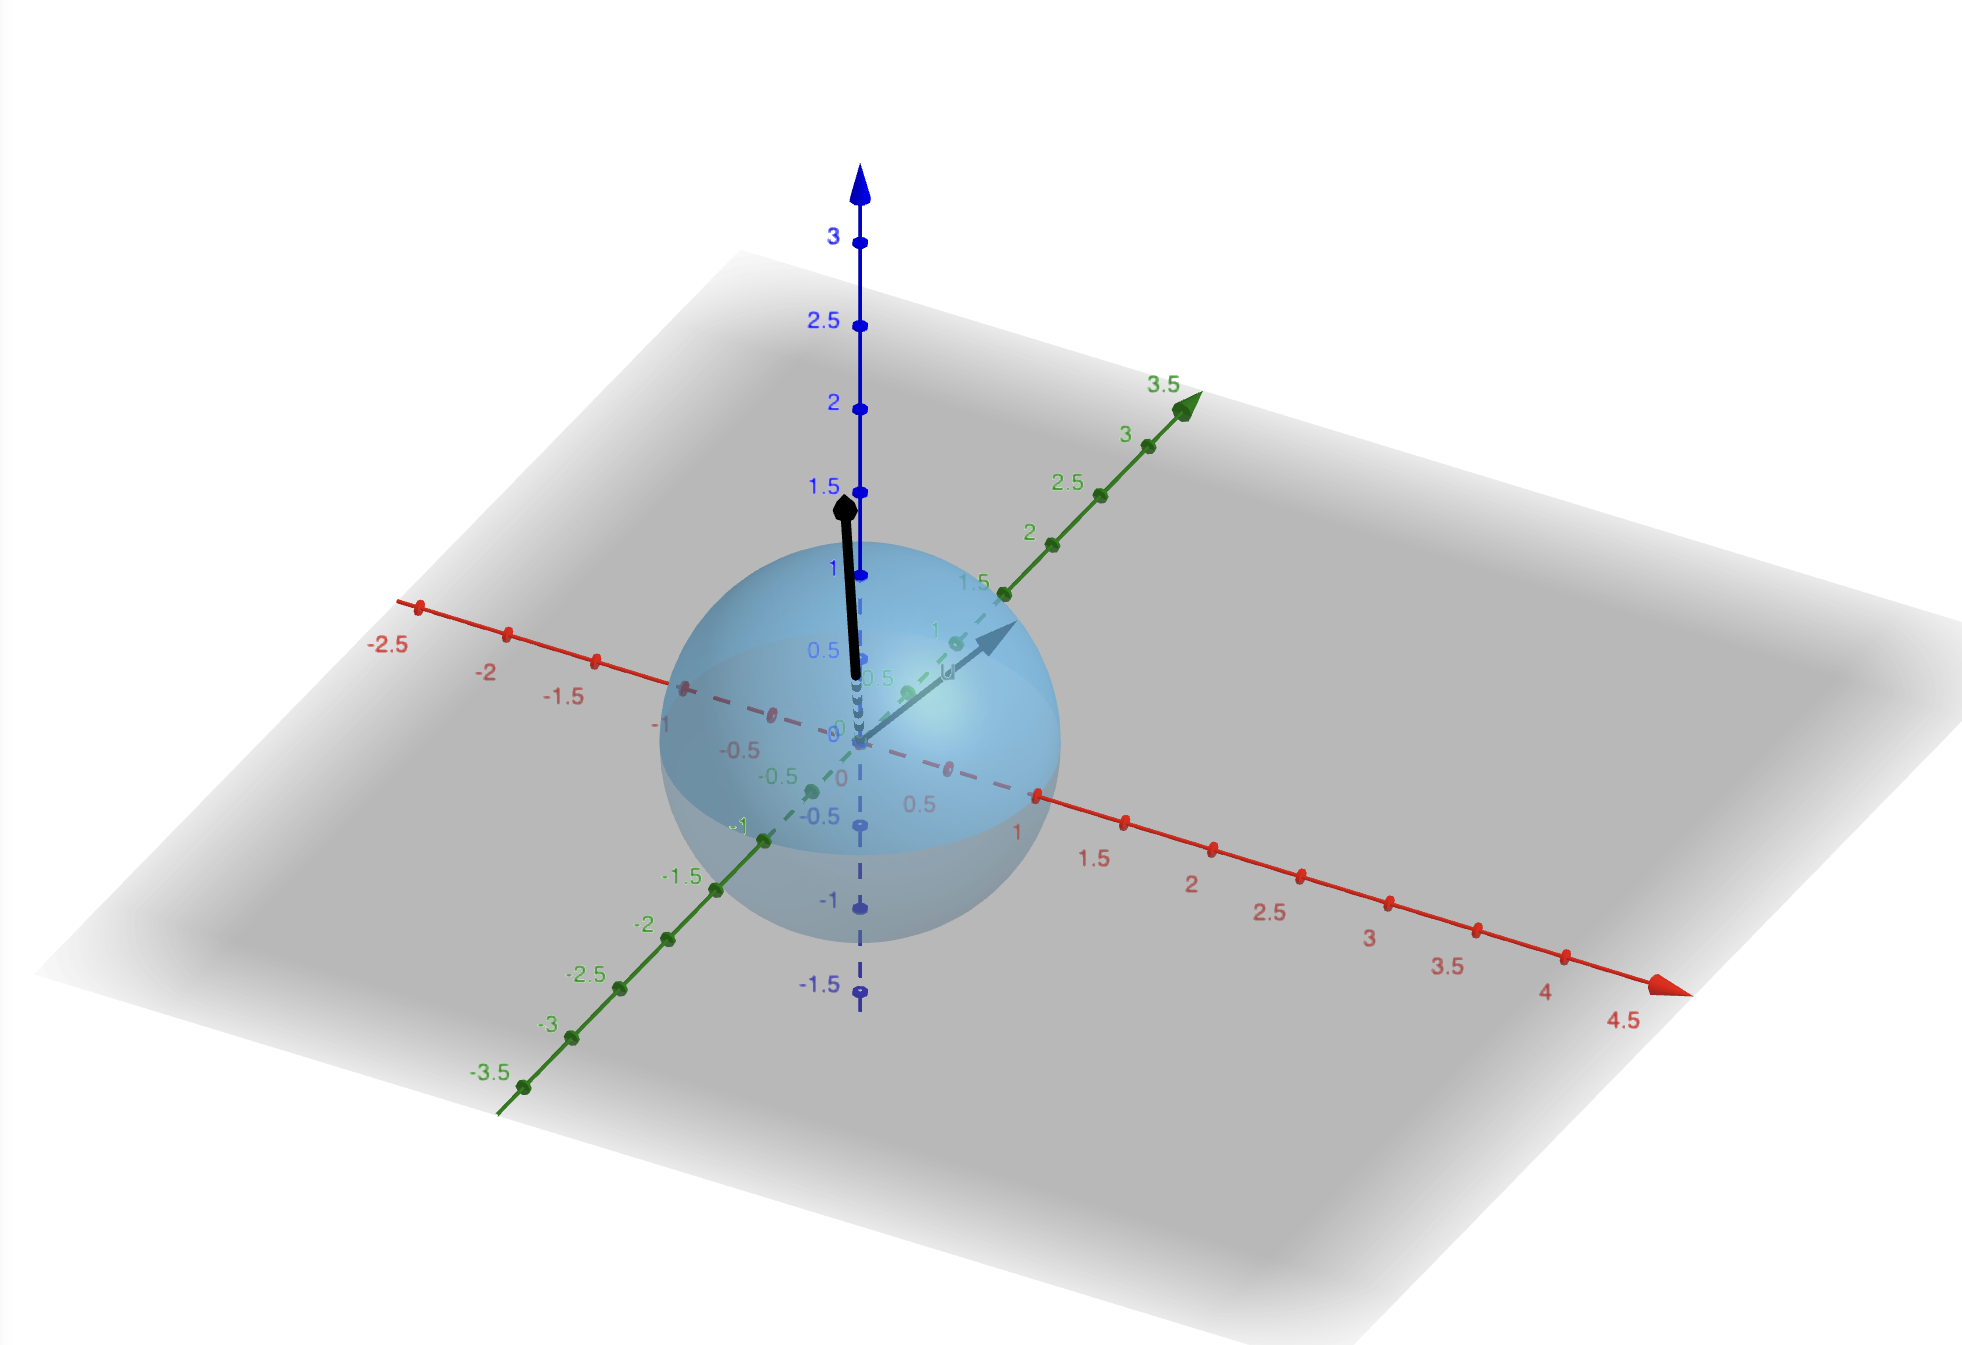
\includegraphics[width = 0.5\textwidth]{vektorji_u_nu}
   \caption{Kvaterniona $\nu$ in $u$ v $\R^3$.}
\end{figure}\\
Ker sta $\nu$ in $u \in \R^3$, skalarni produkt $\dotpr{\nu}{u}$ ustreza kar običajnemu skalarnemu produktu vektorjev $\nu, u$ v $\R^3$.
\begin{align*}
   \dotpr{\nu}{u} &= \nu \cdot u = \frac{1}{\sqrt{3}} (1, -2, 3) \cdot (1,1,1)\\
                  &= \frac{2}{\sqrt{3}},
\end{align*}

\noindent pogledamo še njun vektorski produkt
\begin{align*}
   u \times \nu &= \frac{1}{\sqrt{3}}(1,1,1)\times(1,-2,3)\\
                &= \frac{1}{\sqrt{3}}(5,-2,-3).
\end{align*}

Vstavimo $u$ in $\nu$ ter dobljene rezultate v končo formulo
\begin{align*}
   C\nu &= \dotpr{\nu}{u}(1 - \cos\theta)u + \cos\theta \nu + \sin\theta u\times\nu\\
        &= \frac{2}{\sqrt{3}}(1 - \cos\frac{\pi}{4}) \cdot \frac{1}{\sqrt{3}}(1,1,1) + \cos\frac{\pi}{4}(1,-2,3) + \sin\frac{\pi}{4} \cdot \frac{1}{\sqrt{3}}(5,-2,-3)\\
        &= \frac{2}{3}(1 - \frac{1}{\sqrt{2}})(1,1,1) + \frac{1}{\sqrt{2}}(1,-2,3) + \frac{1}{\sqrt{6}}(5,-2,-3)\\
        &= \big( \frac{4-2\sqrt{2}}{6} + \frac{3\sqrt{2}}{6} + \frac{5\sqrt{6}}{6},\frac{4-2\sqrt{2}}{6} - \frac{6\sqrt{2}}{6} - \frac{2\sqrt{6}}{6}, \frac{4-2\sqrt{2}}{6} + \frac{9\sqrt{2}}{6} - \frac{3\sqrt{6}}{6}\big)\\
        &\approxeq (2.94, -2.04, 1.09).
\end{align*}

\begin{figure}[ht]
   \centering
   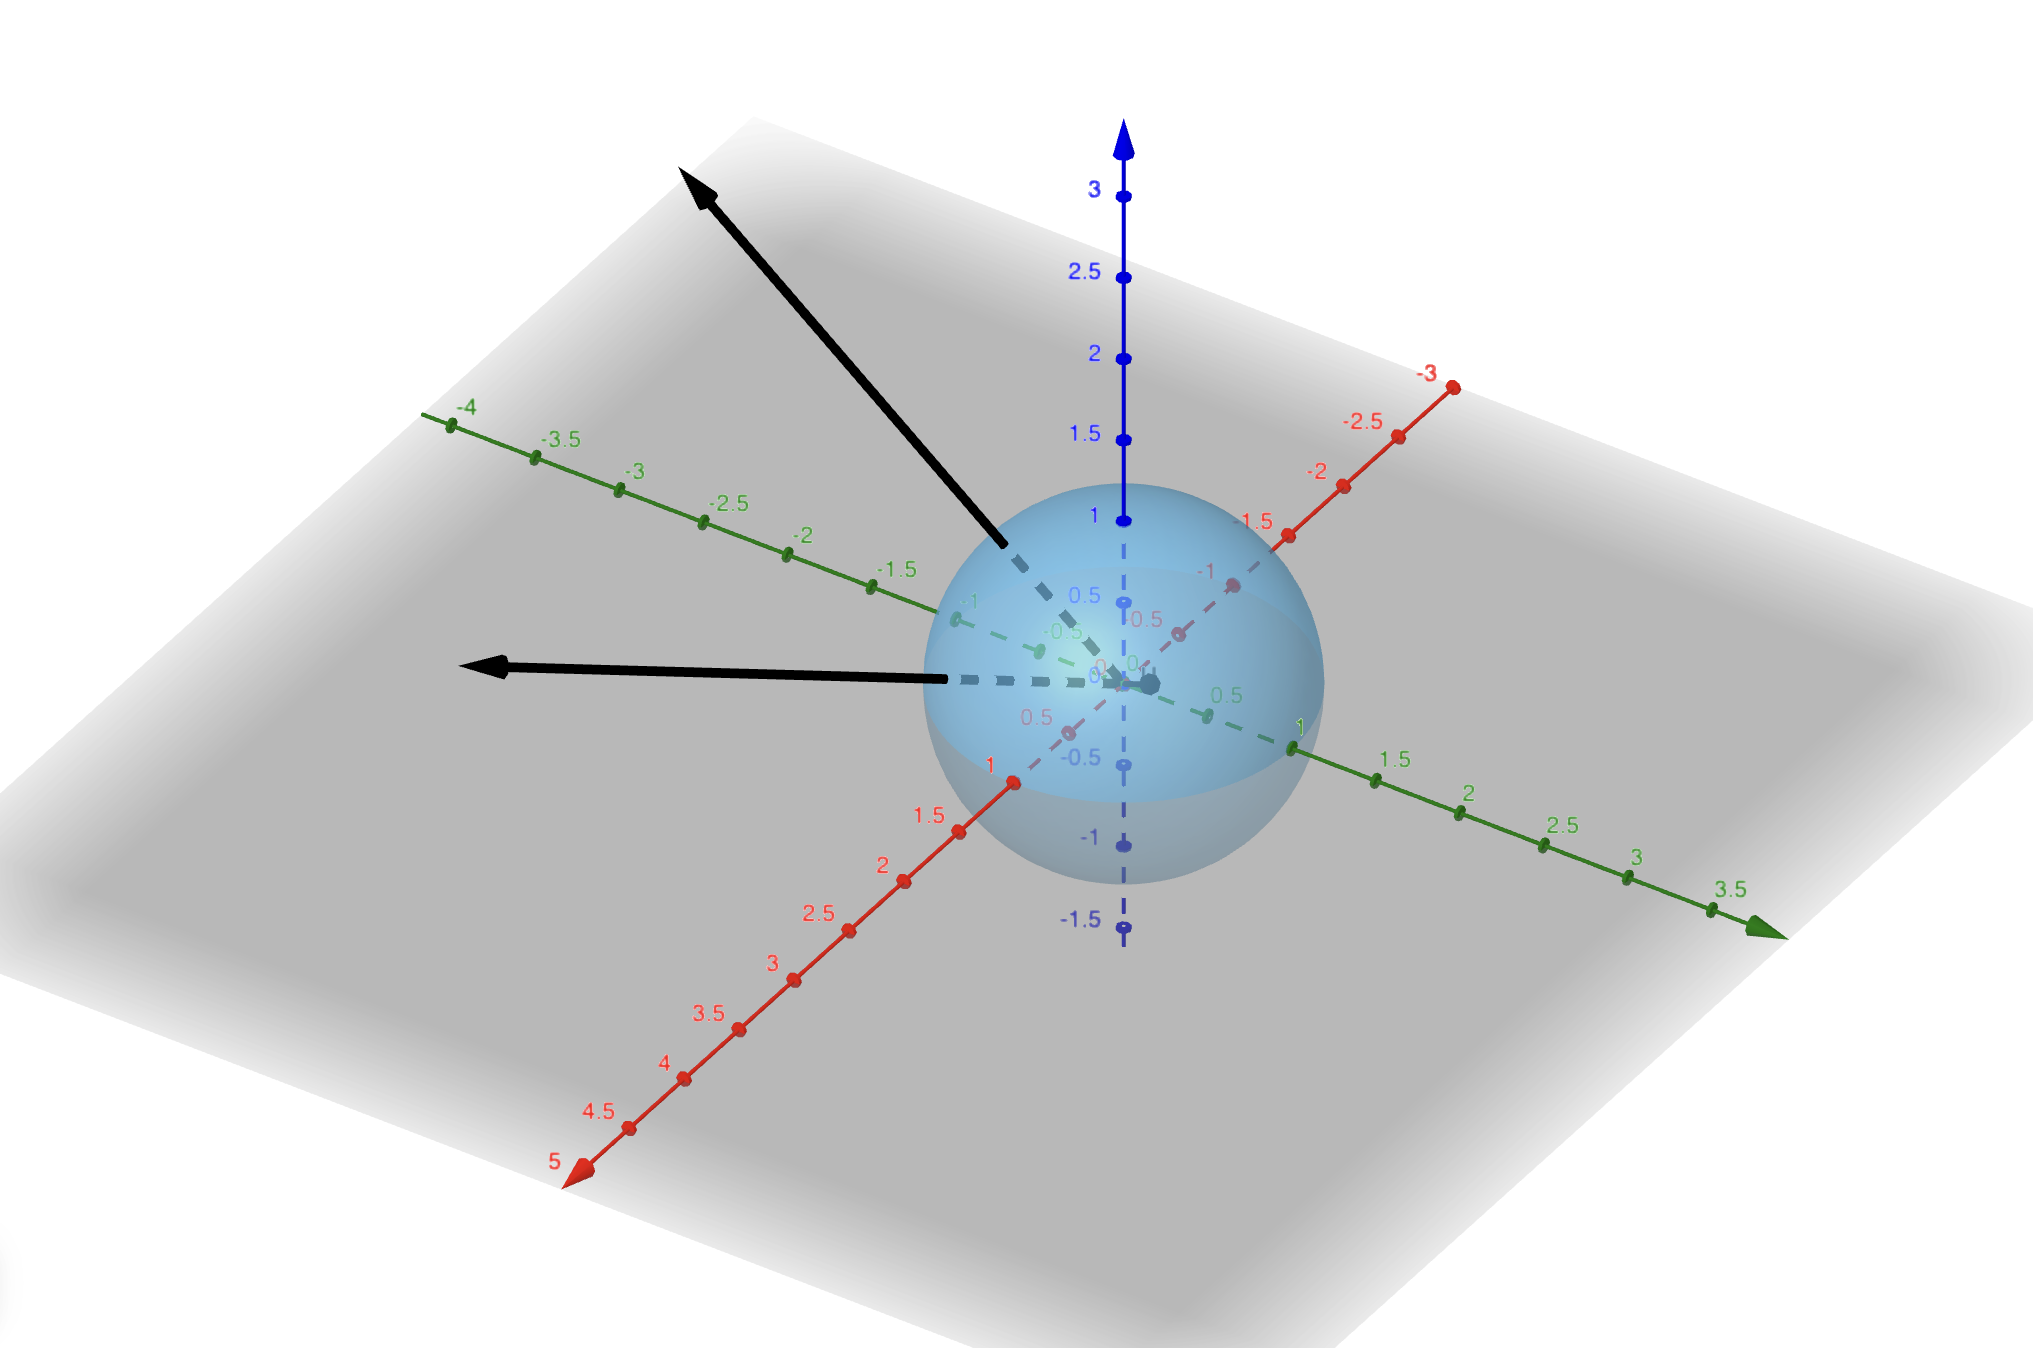
\includegraphics[width = 0.5\textwidth]{vektorji_nu_nu2}
   \caption{Kvaternioni $u$, $\nu$ ter preslikani $\nu$.}
\end{figure}


\newpage


\section*{Angleško-slovenski slovar strokovnih izrazov}

\geslo{Euler's rotation theorem}{Eulerjev izrek o rotacijah}

\geslo{Euler angles}{Eulerjevi koti}

\geslo{transformation}{transformacija, preslikava}

\geslo{matrix}{matrika}

\geslo{origin}{koordinatno izhodišče}

\geslo{quaternion}{kvaternion}

\geslo{dot product}{skalarni produkt}

\geslo{cross product}{vektorski produkt}

\geslo{quaternion conjugate}{konjugirana vrednost kvaterniona}

\geslo{norm}{norma}

\geslo{unit quaternion}{enotski kvaternion}

\geslo{pure quaternion}{pravi oziroma čisti kvaternion}

\geslo{versor}{versor, enotski čisti kvaternion}

\geslo{polar form}{polarni zapis, polarna oblika}

\geslo{orthogonal}{pravokoten}

\geslo{Taylor expansion}{Taylorjev razvoj}

\geslo{uniform convergence}{enakomerna konvergenca}

\geslo{orthogonal transformation}{ortogonalna preslikava}

\geslo{isometry}{izometrija}

\geslo{invariant}{invarianten}

\geslo{span}{linearna ogrinjača}

\geslo{Gram-Schmidt orthogonalisation process}{Gram-Schmidtova ortogonalizacija}


\bibliographystyle{unsrt}
\bibliography{viri}

\end{document}